\section{Dataset}


\subsection{MNIST}
MNIST\cite{LeCunMNISThandwrittendigit2010} is one of the most popular dataset that machine learning partitioners use to benchmark machine learning algorithms. The dataset consists of 60,000 training and 10,000 testing samples. Each sample is a grayscale 28x28 image of a digit between from 0 to 9. 

\begin{figure}[h]
\centering
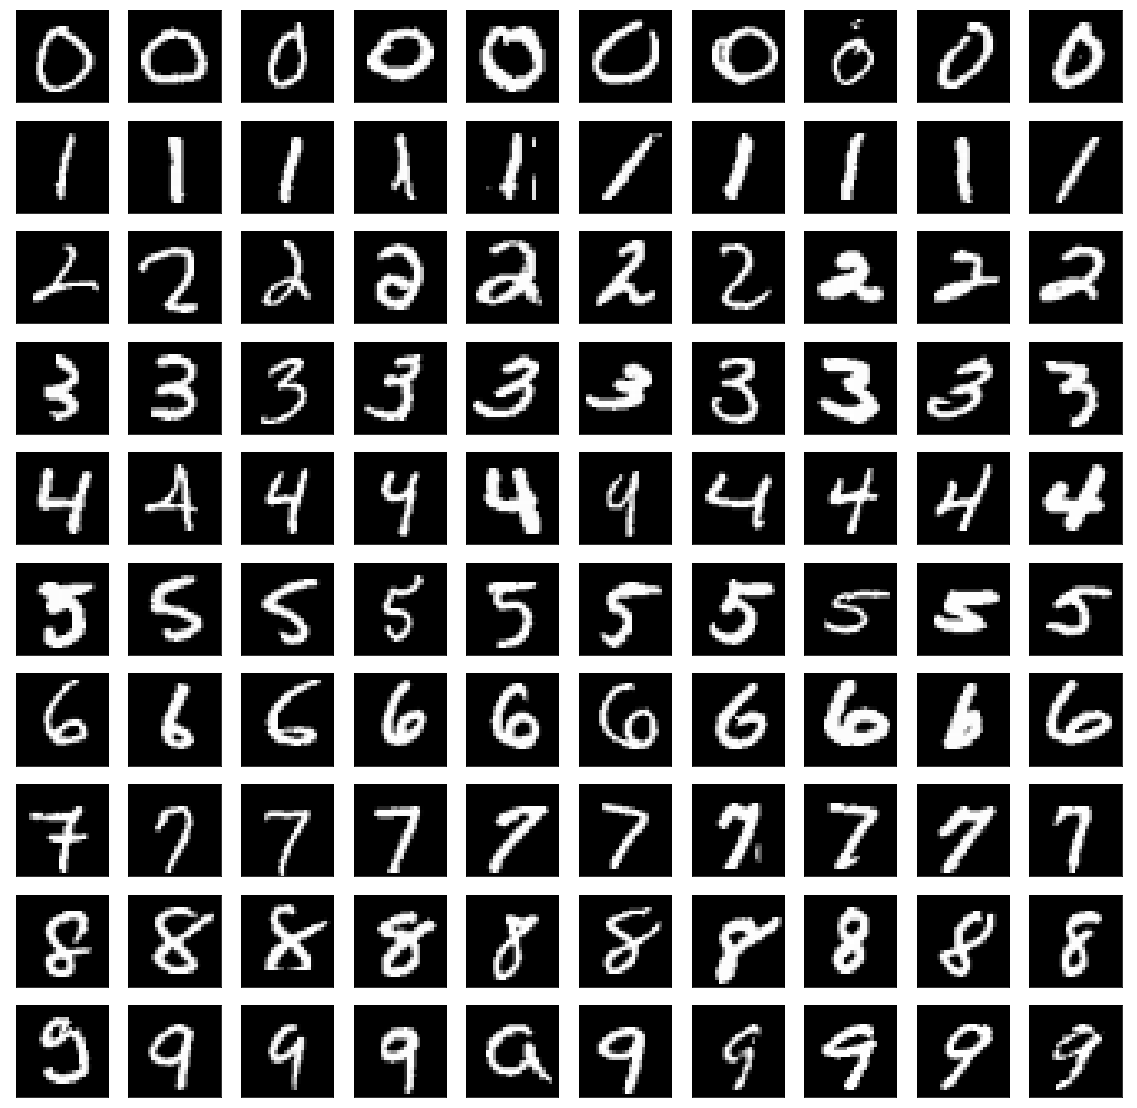
\includegraphics[width=0.5\textwidth]{mnist}
\caption{Samples in MNIST}
\label{fig:mnist_samples}
\end{figure}

State-of-the-art algorithms can classify MNIST with accuracy higher than 0.99, while classical ones, such as SVC or RandomForest, are able to achieve around 0.97\cite{XiaoFashionMNISTNovelImage2017}.


\subsection{FashionMNIST}

Xiao et. al.\cite{XiaoFashionMNISTNovelImage2017} propose a novel dataset, called FashionMNIST dataset, as a replacement of MNIST dataset for benchmarking machine learning algorithms.  According to \cite{XiaoFashionMNISTNovelImage2017},  Fashion-MNIST brings more challenging to the problem and more representative to modern computer vision tasks. It contains images of fashion products from 10 categories. Fashion-MNIST is comparable to MNIST in every aspects, such as the size of training and testing set, image dimension and data format, hence one can easily  apply existing algorithms that work with MNIST to Fashion-MNIST without any change.

\begin{figure}[h]
\centering
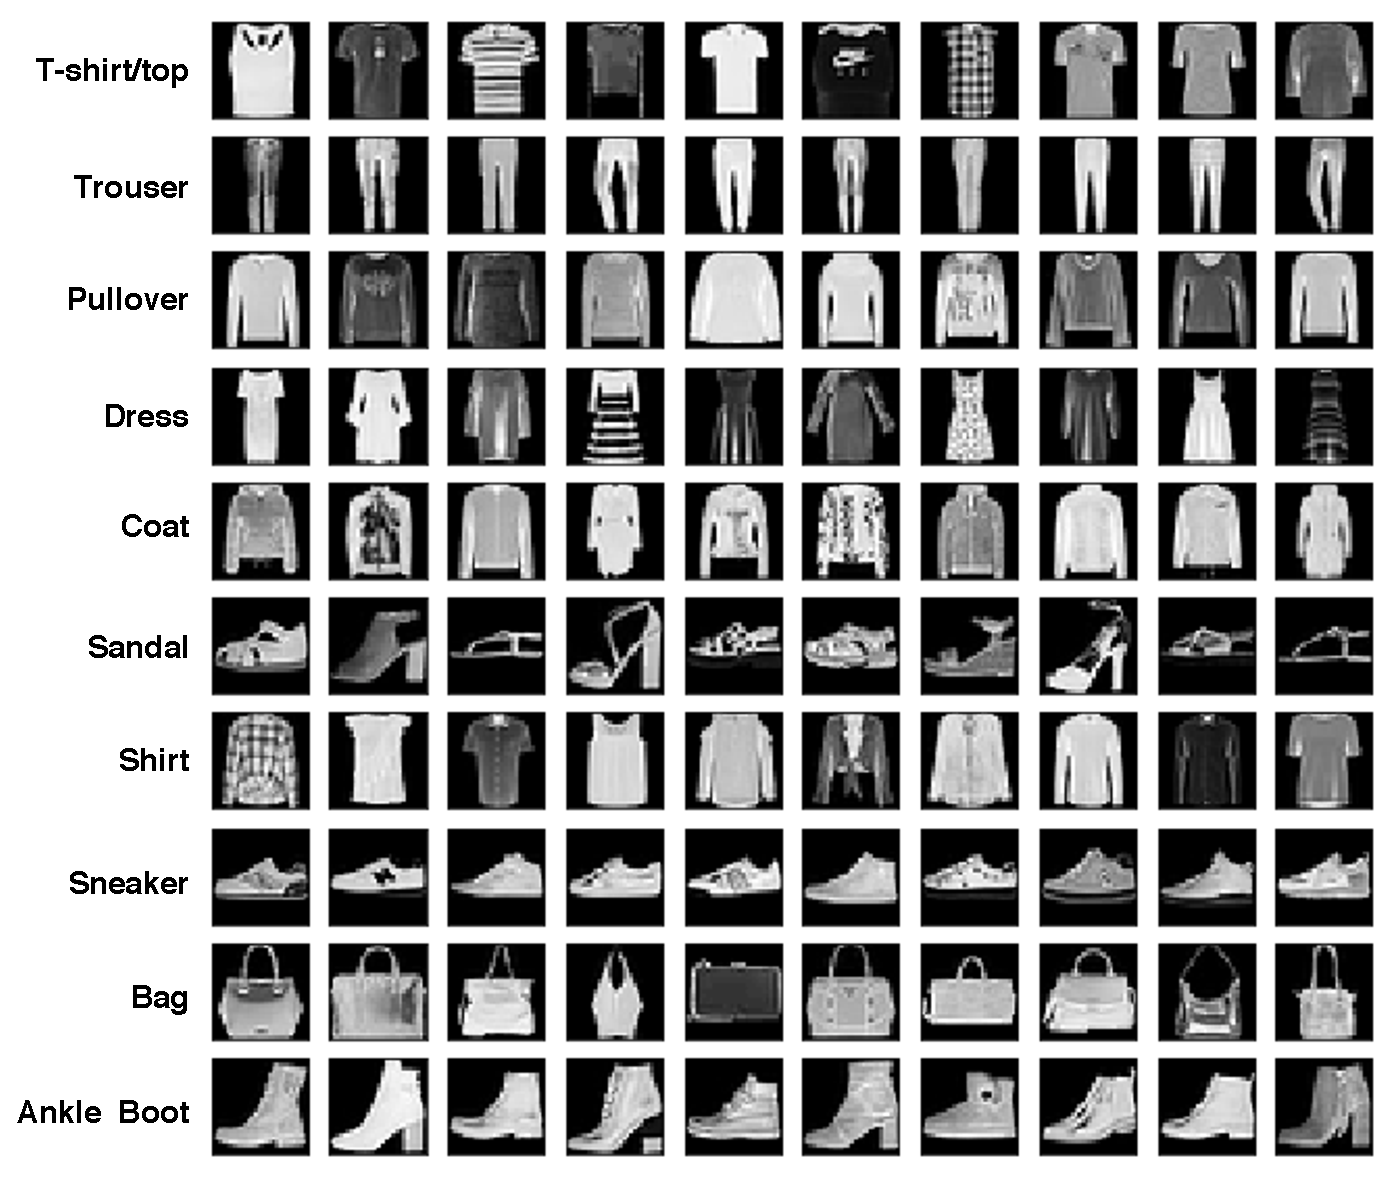
\includegraphics[width=0.6\textwidth]{sketch/fmnist_samples}
\caption{Samples in FashionMNIST}
\label{fig:fashion_mnist_samples}
\end{figure}

\cite{XiaoFashionMNISTNovelImage2017} also reports benchmarking results of classical machine learning algorithms on Fashion-MNIST. On average, they achieve accuracy between 0.85 to 0.89. According to Fashion-MNIST's page\footnote{https://github.com/zalandoresearch/fashion-mnist}, A. Brock reports the state-of-the-art result  with 0.97 accuracy using Wide Residual Network(WRN)\cite{ZagoruykoWideResidualNetworks2016} and standard data preprocessing and augmentation.

